\documentclass[aspectratio=169]{beamer}
\usepackage{beamerstyle}

\begin{document}

% Title slide
\begin{frame}
	\vspace{2cm}
	\begin{center}
		{\Huge\textbf{\textcolor{copenhagenred}{Importance Sampling}}}
		\vspace{1cm}

		\rule{4cm}{3pt}
		\vspace{2cm}
	\end{center}
\end{frame}

% % Slide 1: What, Why, and How
\begin{frame}{What is Importance Sampling?}
	\begin{columns}
		\begin{column}{0.48\textwidth}
			\textbf{What?}
			\begin{itemize}
				\item Monte Carlo technique for estimating $\mathbb{E}_\pi[\phi(X)]$
				\item Sample from proposal $q$ instead of target $\pi$
				\item Reweight samples to correct bias
			\end{itemize}

			\vspace{0.3cm}
			\textbf{Why?}
			\begin{itemize}
				\item Target $\pi$ difficult to sample from
				\item Focus sampling in important regions
				\item Works with unnormalized distributions
				\item All samples are used (unlike rejection)
			\end{itemize}
		\end{column}

		\begin{column}{0.48\textwidth}
			\textbf{How?} The key identity:
			\begin{align*}
				\mathbb{E}_\pi[\phi(X)] & = \int \phi(x)\pi(x)dx                  \\
				                        & = \int \phi(x)\frac{\pi(x)}{q(x)}q(x)dx \\
				                        & = \mathbb{E}_q[\phi(X)w(X)]
			\end{align*}

			\begin{block}{Algorithm}
				\begin{enumerate}
					\item Sample $X_1, \ldots, X_n \sim q$
					\item Compute $w(X_i) = \pi(X_i)/q(X_i)$
					\item Estimate: $\hat{I} = \frac{1}{n}\sum_{i=1}^n \phi(X_i)w(X_i)$
				\end{enumerate}
			\end{block}
		\end{column}
	\end{columns}
\end{frame}

% Slide 2: Properties and Unnormalized Distributions
\begin{frame}{Key Properties and Unnormalized Distributions}
	\begin{columns}
		\begin{column}{0.5\textwidth}
			\textbf{Properties of IS Estimator:}
			\begin{itemize}
				\item \textbf{Unbiased}: $\mathbb{E}_q[\hat{I}] = \mathbb{E}_\pi[\phi(X)]$
				\item \textbf{Consistent}: $\hat{I} \xrightarrow{n\to\infty} \mathbb{E}_\pi[\phi(X)]$ (LLN)
				\item \textbf{Variance}: $\text{Var}_q[\hat{I}] = \frac{1}{n}\text{Var}_q[\phi(X)w(X)]$
			\end{itemize}

			\vspace{0.3cm}
			\textbf{Requirements:}
			\begin{itemize}
				\item $q(x) > 0$ whenever $\pi(x)\phi(x) \neq 0$
				\item $\mathbb{E}_q[|\phi(X)w(X)|] < \infty$
			\end{itemize}
		\end{column}

		\begin{column}{0.5\textwidth}
			\textbf{Unnormalized Distributions:}\\
			When $\pi(x) = \tilde{\pi}(x)/Z$ with unknown $Z$:

			\begin{block}{Self-Normalized IS}
				\begin{itemize}
					\item Weights: $\tilde{w}(x) = \tilde{\pi}(x)/q(x)$
					\item Estimator: $$\hat{I}_{SN} = \frac{\sum_{i=1}^n \phi(X_i)\tilde{w}(X_i)}{\sum_{i=1}^n \tilde{w}(X_i)}$$
					\item Biased but consistent
					\item Bias: $O(1/n)$
				\end{itemize}
			\end{block}
		\end{column}
	\end{columns}
\end{frame}

% Slide 3: Weight Distribution and ESS
\begin{frame}{Why Weight Distribution Matters }
			\textbf{Weight Distribution Impact:}
			\begin{itemize}
				\item High weight variance $\Rightarrow$ poor estimates
				\item Few samples dominate the sum
				\item Ideal case: all weights equal ($q = \pi$)
				\item $\text{Var}_q[w(X)]$ determines convergence
			\end{itemize}

			\vspace{0.3cm}
			\textbf{Example Weight Degeneracy:}
			\begin{center}
				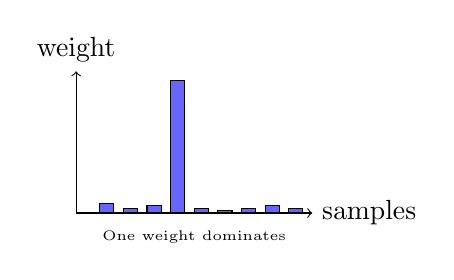
\begin{tikzpicture}[scale=0.6]
					\draw[->] (0,0) -- (5,0) node[right] {samples};
					\draw[->] (0,0) -- (0,3) node[above] {weight};
					\foreach \x/\y in {0.5/0.2, 1/0.1, 1.5/0.15, 2/2.8, 2.5/0.1, 3/0.05, 3.5/0.1, 4/0.15, 4.5/0.1}
					\draw[fill=blue!60] (\x,0) rectangle (\x+0.3,\y);
					\node at (2.5,-0.5) {\tiny One weight dominates};
				\end{tikzpicture}
			\end{center}
	
\end{frame}

\begin{frame}{Effective Sample Size (ESS)}
		\begin{block}{Definition}
			$$\text{ESS} = \frac{(\sum_{i=1}^n w_i)^2}{\sum_{i=1}^n w_i^2}$$
		\end{block}

		\textbf{Interpretation:}
		\begin{itemize}
			\item Number of "equivalent" samples from $\pi$
			\item Range: $1 \leq \text{ESS} \leq n$
			\item ESS $= n$ when all weights equal, ESS $= 1$ when one weight dominates
		\end{itemize}

		\textbf{Why ESS Matters:}
		\begin{itemize}
			\item ESS $\ll n$ indicates weight degeneracy
			\item Low ESS $\Rightarrow$ high variance
			\item Monitor ESS to diagnose problems
			\item Rule of thumb: ESS $> n/2$ is good
		\end{itemize}
\end{frame}

% Slide 4: Choosing Proposal and Dimensional Scaling
\begin{frame}{Choosing Good Proposals \& Dimensional Scaling}
	\begin{columns}
		\begin{column}{0.5\textwidth}
			\textbf{Good Proposal Properties:}
			\begin{enumerate}
				\item Heavier tails than $\pi$
				\item Easy to sample from
				\item Similar shape to $\pi|\phi|$
				\item Covers support of $\pi$
				\item Minimizes $\text{Var}_q[\phi(X)w(X)]$
			\end{enumerate}

			\vspace{0.3cm}
			\textbf{Common Choices:}
			\begin{itemize}
				\item Student-t for Gaussian targets
				\item Mixture distributions
				\item Previous MCMC output
				\item Laplace approximation
			\end{itemize}
		\end{column}

		\begin{column}{0.5\textwidth}
			\textbf{Curse of Dimensionality:}
			\begin{block}{Gaussian Example}
				For $\pi = \mathcal{N}(0,I_d)$, $q = \mathcal{N}(0,\sigma^2 I_d)$:
				$$\text{Var}_q[w(X)] = \left(\frac{\sigma^4}{2\sigma^2-1}\right)^{d/2} - 1$$
			\end{block}

			\textbf{Numerical Example:}
			\begin{center}
				\begin{tabular}{ccc}
					% \toprule
					$d$ & $\sigma$ & $\text{Var}_q[w(X)]$               \\
					% \midrule
					10  & 1.2      & $\approx 5.6$                      \\
					50  & 1.2      & $\approx 850$                      \\
					100 & 1.2      & $\approx \mathbf{1.8 \times 10^4}$ \\
					% \bottomrule
				\end{tabular}
			\end{center}

			\textbf{Variance explodes exponentially!}
		\end{column}
	\end{columns}
\end{frame}

% Slide 5: Comparison with Rejection Sampling
\begin{frame}{Importance Sampling vs. Rejection Sampling}
	\begin{center}
		\small
		\begin{tabular}{lll}
			% \toprule
			\textbf{Aspect}             & \textbf{Importance Sampling}   & \textbf{Rejection Sampling}     \\
			% \midrule
			\textbf{Sample usage}       & All samples (weighted)         & Some samples rejected           \\
			\textbf{Efficiency}         & Depends on weight variance     & Depends on acceptance rate      \\
			\textbf{High dimensions}    & Poor (variance explodes)       & Very poor (accept rate $\to 0$) \\
			\textbf{Proposal req.}      & $q > 0$ where $\pi\phi \neq 0$ & Need $Mq \geq \pi$ everywhere   \\
			\textbf{Output}             & Weighted samples               & Exact samples from $\pi$        \\
			\textbf{Normalizing const.} & Not required                   & Required (for bound $M$)        \\
			\textbf{Bias}               & Unbiased (or consistent)       & Unbiased (exact)                \\
			\textbf{Failure mode}       & High variance                  & No samples produced             \\
			% \bottomrule
		\end{tabular}
	\end{center}

	\vspace{0.5cm}
	\begin{block}{Key Insight}
		Both methods suffer from curse of dimensionality, but:
		\begin{itemize}
			\item IS degrades gracefully - still provides estimates (with high variance)
			\item Rejection sampling can fail completely - may produce no samples
			\item IS better for moderate dimensions and when $\pi$ known up to constant
		\end{itemize}
	\end{block}
\end{frame}

% % Summary Slide
% \begin{frame}{Summary: Best Practices}
% 	\begin{columns}
% 		\begin{column}{0.5\textwidth}
% 			\textbf{Strengths:}
% 			\begin{itemize}
% 				\item[\checkmark] Handles complex distributions
% 				\item[\checkmark] Unbiased estimates
% 				\item[\checkmark] Works with unnormalized $\pi$
% 				\item[\checkmark] All samples contribute
% 				\item[\checkmark] Flexible proposal choice
% 			\end{itemize}

% 			\vspace{0.3cm}
% 			\textbf{Limitations:}
% 			\begin{itemize}
% 				\item[$\times$] Curse of dimensionality
% 				\item[$\times$] Sensitive to proposal choice
% 				\item[$\times$] Weight degeneracy issues
% 				\item[$\times$] Can have infinite variance
% 			\end{itemize}
% 		\end{column}

% 		\begin{column}{0.5\textwidth}
% 			\textbf{Best Practices:}
% 			\begin{enumerate}
% 				\item \textbf{Monitor ESS} regularly
% 				\item \textbf{Check weight distribution} for outliers
% 				\item \textbf{Use heavy-tailed proposals} (e.g., $t$-distribution)
% 				\item \textbf{Consider adaptive IS} to improve $q$
% 				\item \textbf{Multiple IS} for robustness
% 				\item \textbf{Diagnostic plots}: weights, ESS over time
% 			\end{enumerate}

% 			\vspace{0.3cm}
% 			\begin{block}{Rule of Thumb}
% 				If ESS $< n/10$, reconsider your proposal!
% 			\end{block}
% 		\end{column}
% 	\end{columns}
% \end{frame}

\end{document}